
\documentclass[tikz,border=5pt]{standalone}
\usepackage[T1]{fontenc}
\usepackage{newtxtext,newtxmath}
\usepackage{tikz}
\usetikzlibrary{arrows.meta,positioning,fit,calc}
\definecolor{oasiblue}{RGB}{45,82,122}
\definecolor{oasigreen}{RGB}{63,108,79}
\definecolor{oasiorange}{RGB}{150,92,40}
\definecolor{oasigray}{RGB}{84,91,99}
\begin{document}
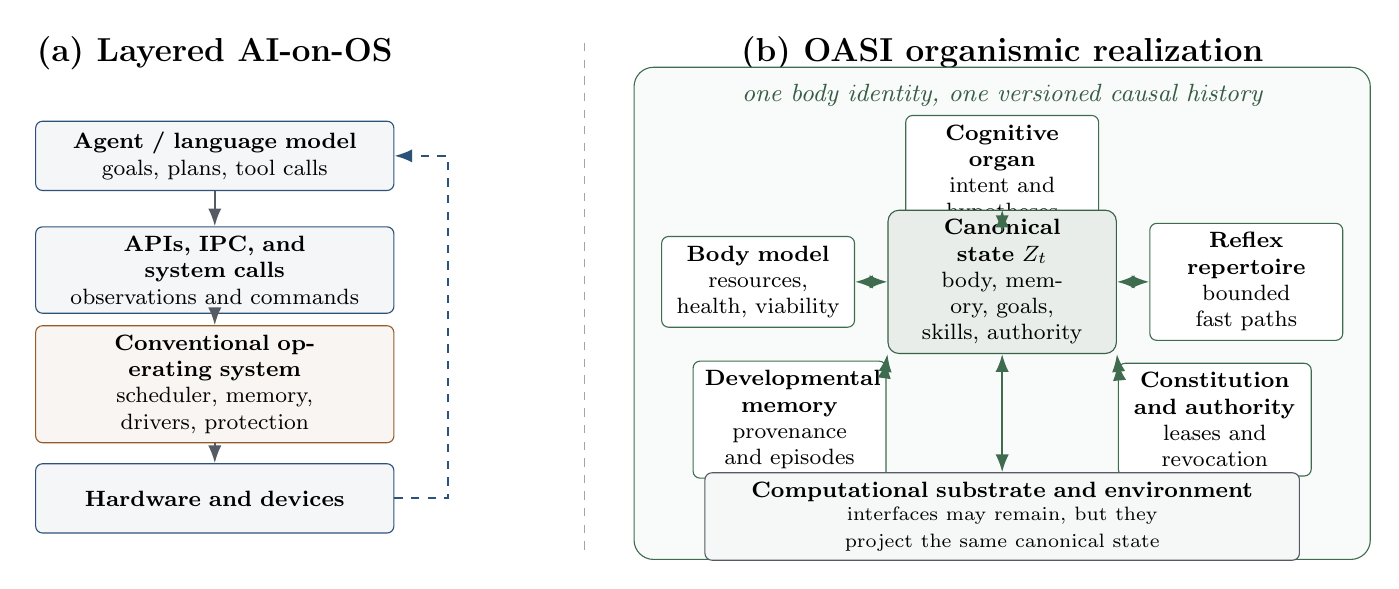
\begin{tikzpicture}[
  font=\footnotesize, >=Latex,
  layer/.style={draw=oasiblue,rounded corners=2.5pt,fill=oasiblue!5,
    minimum width=4.55cm,text width=4.10cm,minimum height=.88cm,align=center},
  oslayer/.style={draw=oasiorange,rounded corners=2.5pt,fill=oasiorange!6,
    minimum width=4.55cm,text width=4.10cm,minimum height=.92cm,align=center},
  organ/.style={draw=oasigreen,rounded corners=2.5pt,fill=white,
    minimum width=2.45cm,text width=2.15cm,minimum height=.86cm,align=center},
  hub/.style={draw=oasigreen!90!black,rounded corners=4pt,fill=oasigreen!12,
    minimum width=2.90cm,text width=2.62cm,minimum height=1.08cm,align=center},
  substrate/.style={draw=oasigray,rounded corners=2.5pt,fill=oasigray!5,
    minimum width=7.55cm,text width=7.10cm,minimum height=.82cm,align=center},
  arr/.style={->,line width=.76pt,draw=oasigray},
  bi/.style={Latex-Latex,line width=.76pt,draw=oasigreen}
]
\node[font=\bfseries\large] at (-4.55,3.25) {(a) Layered AI-on-OS};
\node[font=\bfseries\large] at (5.45,3.25) {(b) OASI organismic realization};

\node[layer] (agent) at (-4.55,1.95) {\textbf{Agent / language model}\\goals, plans, tool calls};
\node[layer] (api) at (-4.55,.50) {\textbf{APIs, IPC, and system calls}\\observations and commands};
\node[oslayer] (os) at (-4.55,-.95) {\textbf{Conventional operating system}\\scheduler, memory, drivers, protection};
\node[layer] (hw) at (-4.55,-2.40) {\textbf{Hardware and devices}};
\draw[arr] (agent) -- (api);
\draw[arr] (api) -- (os);
\draw[arr] (os) -- (hw);
\draw[arr,dashed,draw=oasiblue] (hw.east) -- ++(.68,0) |- (agent.east);

\draw[dashed,draw=oasigray!55] (.15,-3.05) -- (.15,3.38);

\node[draw=oasigreen,rounded corners=7pt,fill=oasigreen!3,
      minimum width=9.35cm,minimum height=6.25cm] (frame) at (5.45,-.05) {};
\node[font=\itshape\small,text=oasigreen!85!black] at (5.45,2.72)
 {one body identity, one versioned causal history};

\node[organ] (cog) at (5.45,1.72) {\textbf{Cognitive organ}\\intent and hypotheses};
\node[organ] (body) at (2.35,.35) {\textbf{Body model}\\resources, health, viability};
\node[hub] (state) at (5.45,.35) {\textbf{Canonical state} $Z_t$\\body, memory, goals,\\skills, authority};
\node[organ] (reflex) at (8.55,.35) {\textbf{Reflex repertoire}\\bounded fast paths};
\node[organ] (memory) at (2.75,-1.40) {\textbf{Developmental memory}\\provenance and episodes};
\node[organ] (authority) at (8.15,-1.40) {\textbf{Constitution and authority}\\leases and revocation};

\draw[bi] (cog.south) -- (state.north);
\draw[bi] (body.east) -- (state.west);
\draw[bi] (reflex.west) -- (state.east);
\draw[bi] (memory.north east) -- (state.south west);
\draw[bi] (authority.north west) -- (state.south east);

\node[substrate] (substrate) at (5.45,-2.63)
 {\textbf{Computational substrate and environment}\\[-1pt]
  \scriptsize interfaces may remain, but they project the same canonical state};
\draw[bi] (state.south) -- (substrate.north);
\end{tikzpicture}
\end{document}
